% ══════════════════════════════════════════════════════════════════
% ANNEXES A — B — C — D
% ══════════════════════════════════════════════════════════════════

\chapter{Jeux de données utilisés}
\label{ann:datasets}

\section*{A.1 --- Dataset Irrigation (NASA POWER)}

\begin{table}[H]
	\centering
	\caption{Caractéristiques du dataset d'irrigation}
	\label{tab:ann_irr}
	\begin{tabularx}{\textwidth}{lX}
		\toprule
		\textbf{Caractéristique} & \textbf{Valeur} \\
		\midrule
		Source          & NASA POWER (power.larc.nasa.gov) \\
		Période         & 2015--2023 \\and Zhang, Taiping and
		Westberg, David and others},
		title   = {{NASA POWER}: Prediction Of Worldwi
		Observations    & 16~435 \\
		Variables       & 15 explicatives + 1 cible binaire \\
		Villes          & N'Djamena, Abéché, Sarh, Moundou, Bongor \\
		Cultures        & Mil, Sorgho, Arachide, Maïs, Coton \\
		Cible           & Besoin en irrigation (OUI / NON) \\
		\bottomrule
	\end{tabularx}
\end{table}

\section*{A.2 --- Dataset Fertilisation}

\begin{table}[H]
	\centering
	\caption{Caractéristiques du dataset de fertilisation}
	\label{tab:ann_fert}
	\begin{tabularx}{\textwidth}{lX}
		\toprule
		\textbf{Caractéristique} & \textbf{Valeur} \\
		\midrule
		Sources         & Dataset public Kaggle (99 obs. réelles)
		+ augmentation cohérente (1~500 obs.) \\
		Observations    & 1~599 \\
		Variables       & N, P, K, pH, température, humidités, pluie,
		culture, type de sol, zone \\
		Classes (5)     & Urée, DAP, NPK 15-15-15, NPK 23-10-5, KCl \\
		\bottomrule
	\end{tabularx}
\end{table}

\section*{A.3 --- Dataset local d'images (maladies)}

\begin{table}[H]
	\centering
	\caption{Distribution du dataset local tchadien (287 images)}
	\label{tab:ann_mal}
	\begin{tabularx}{\textwidth}{lXc}
		\toprule
		\textbf{Classe} & \textbf{Description} & \textbf{Images} \\
		\midrule
		Arachide malade  & Feuilles d'arachide malades  & 28 \\
		Arachide saine   & Feuilles d'arachide saines   & 40 \\
		Coton malade     & Feuilles de coton malades    & 30 \\
		Coton sain       & Feuilles de coton saines     & 26 \\
		Maïs malade      & Feuilles de maïs malades     & 27 \\
		Maïs sain        & Feuilles de maïs saines      & 27 \\
		Mil malade       & Feuilles de mil malades      & 35 \\
		Mil sain         & Feuilles de mil saines       & 23 \\
		Sorgho malade    & Feuilles de sorgho malades   & 27 \\
		Sorgho sain      & Feuilles de sorgho saines    & 24 \\
		\midrule
		\textbf{Total}   & \textbf{10 classes}          & \textbf{287} \\
		\bottomrule
	\end{tabularx}
\end{table}

% ══════════════════════════════════════════════════════════════════
\chapter{Codes sources principaux}
\label{ann:codes}

\section*{B.1 --- Inférence du CNN au format TFLite}

\begin{lstlisting}[language=Python,
	caption={Chargement et inférence du modèle TFLite},
	label={lst:ann_tflite}]
	import numpy as np, json
	import tflite_runtime.interpreter as tflite
	
	interpreter = tflite.Interpreter(
	model_path="models/model_maladie.tflite")
	interpreter.allocate_tensors()
	classes = json.load(
	open("models/config_maladies.json"))["classes"]
	
	def predire(image_pil):
	img = image_pil.convert("RGB").resize((224, 224))
	arr = np.expand_dims(
	np.array(img, dtype=np.float32) / 255.0, 0)
	inp = interpreter.get_input_details()
	out = interpreter.get_output_details()
	interpreter.set_tensor(inp[0]["index"], arr)
	interpreter.invoke()
	preds = interpreter.get_tensor(out[0]["index"])[0]
	i = int(np.argmax(preds))
	return classes[i], float(preds[i]) * 100
\end{lstlisting}

\section*{B.2 --- Statistiques du module Historique}

\begin{lstlisting}[language=Python,
	caption={Calcul des statistiques globales de l'historique},
	label={lst:ann_stats}]
	def statistiques():
	conn = sqlite3.connect("historique.db")
	n_irr  = conn.execute(
	"SELECT COUNT(*) FROM irrigation").fetchone()[0]
	n_fert = conn.execute(
	"SELECT COUNT(*) FROM fertilisation").fetchone()[0]
	n_mal  = conn.execute(
	"SELECT COUNT(*) FROM maladies").fetchone()[0]
	top = conn.execute("""
	SELECT culture, COUNT(*) AS n FROM (
	SELECT culture FROM irrigation
	UNION ALL SELECT culture FROM fertilisation
	UNION ALL SELECT culture FROM maladies)
	GROUP BY culture ORDER BY n DESC LIMIT 1
	""").fetchone()
	conn.close()
	return {"total": n_irr + n_fert + n_mal,
		"culture_top": top[0] if top else "-"}
\end{lstlisting}

\section*{B.3 --- Export CSV}

\begin{lstlisting}[language=Python,
	caption={Export CSV d'une table de l'historique (Streamlit)},
	label={lst:ann_csv}]
	import pandas as pd, streamlit as st
	
	df  = pd.DataFrame(lire_historique_irrigation(1000))
	csv = df.to_csv(index=False).encode("utf-8")
	st.download_button(
	label="Exporter en CSV",
	data=csv,
	file_name="historique_irrigation.csv",
	mime="text/csv")
\end{lstlisting}

% ══════════════════════════════════════════════════════════════════
\chapter{Diagrammes UML complets}
\label{ann:uml}

Les diagrammes UML détaillés (cas d'utilisation avec relations
\textit{include}, diagrammes de séquence des quatre modules,
diagramme de classes complet) sont disponibles dans le dépôt du
projet \cite{agroiatchad2026} :

\begin{center}
	\url{https://github.com/tourabiissakhissein33-dev/PFE_Agriculture_IA}
\end{center}

% ══════════════════════════════════════════════════════════════════
\chapter{Captures d'écran de l'application}
\label{ann:captures}

Les figures ci-dessous présentent les principales interfaces de
l'application.

\begin{figure}[H]
	\centering
	% 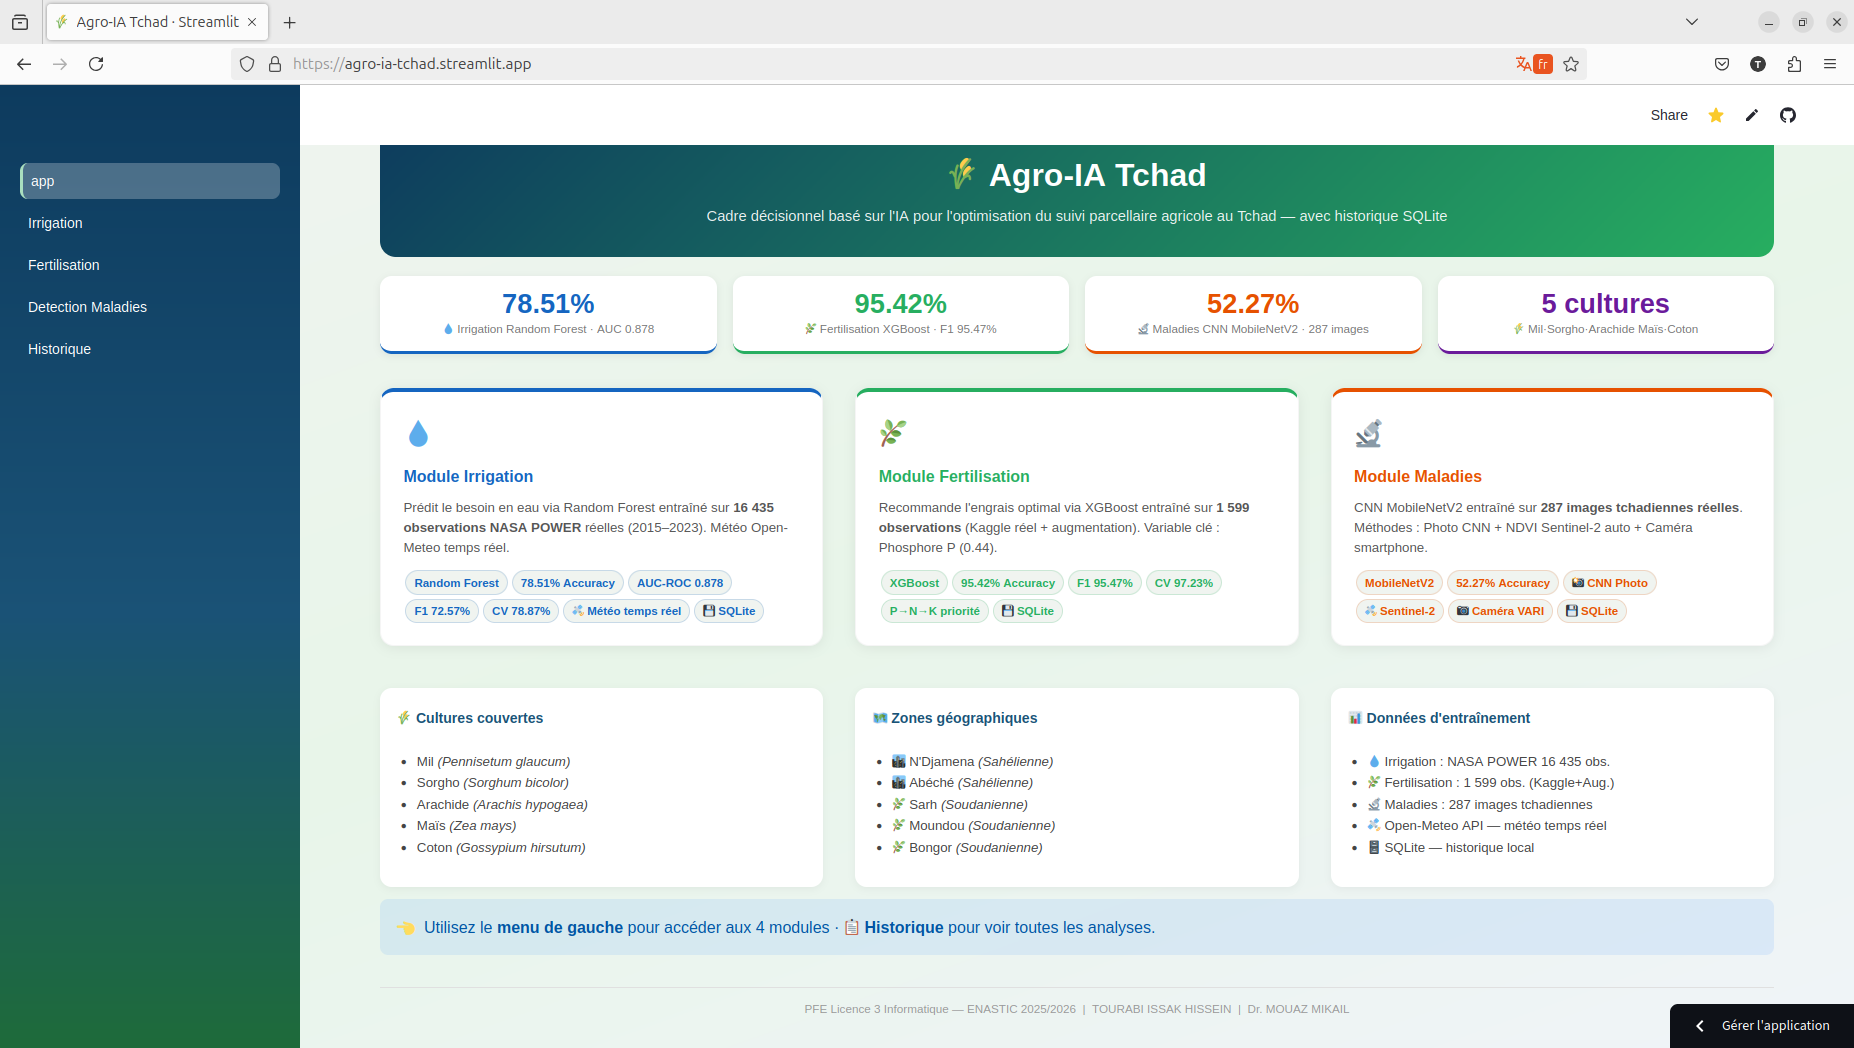
\includegraphics[width=0.9\textwidth]{images/capture_accueil.png}
	\fbox{\parbox{0.9\textwidth}{\centering\vspace{1.4cm}
			[Capture : page d'accueil --- métriques et statistiques]
			\vspace{1.4cm}}}
	\caption{Page d'accueil de l'application Agro-IA Tchad}
	\label{fig:cap_accueil}
\end{figure}

\begin{figure}[H]
	\centering
	% 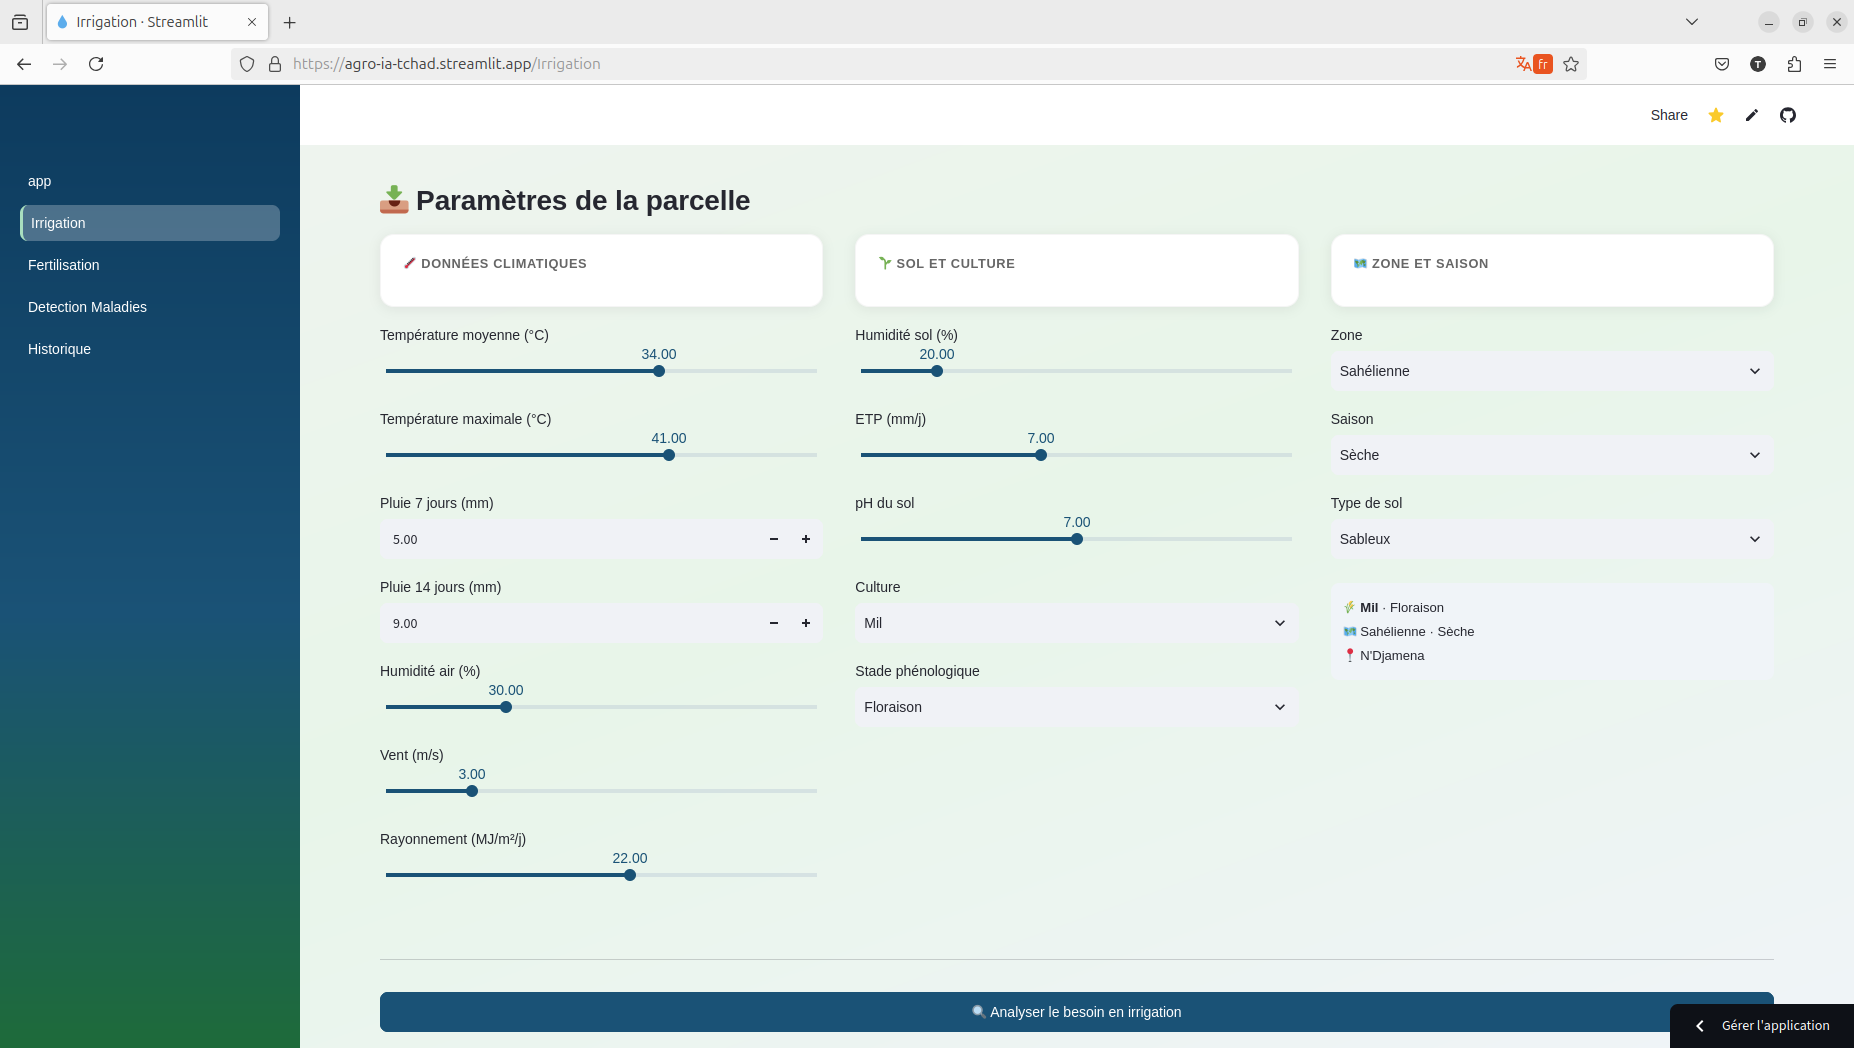
\includegraphics[width=0.9\textwidth]{images/capture_irrigation.png}
	\fbox{\parbox{0.9\textwidth}{\centering\vspace{1.4cm}
			[Capture : module Irrigation --- météo temps réel et résultat]
			\vspace{1.4cm}}}
	\caption{Module Irrigation --- analyse et recommandation}
	\label{fig:cap_irr}
\end{figure}

\begin{figure}[H]
	\centering
	% 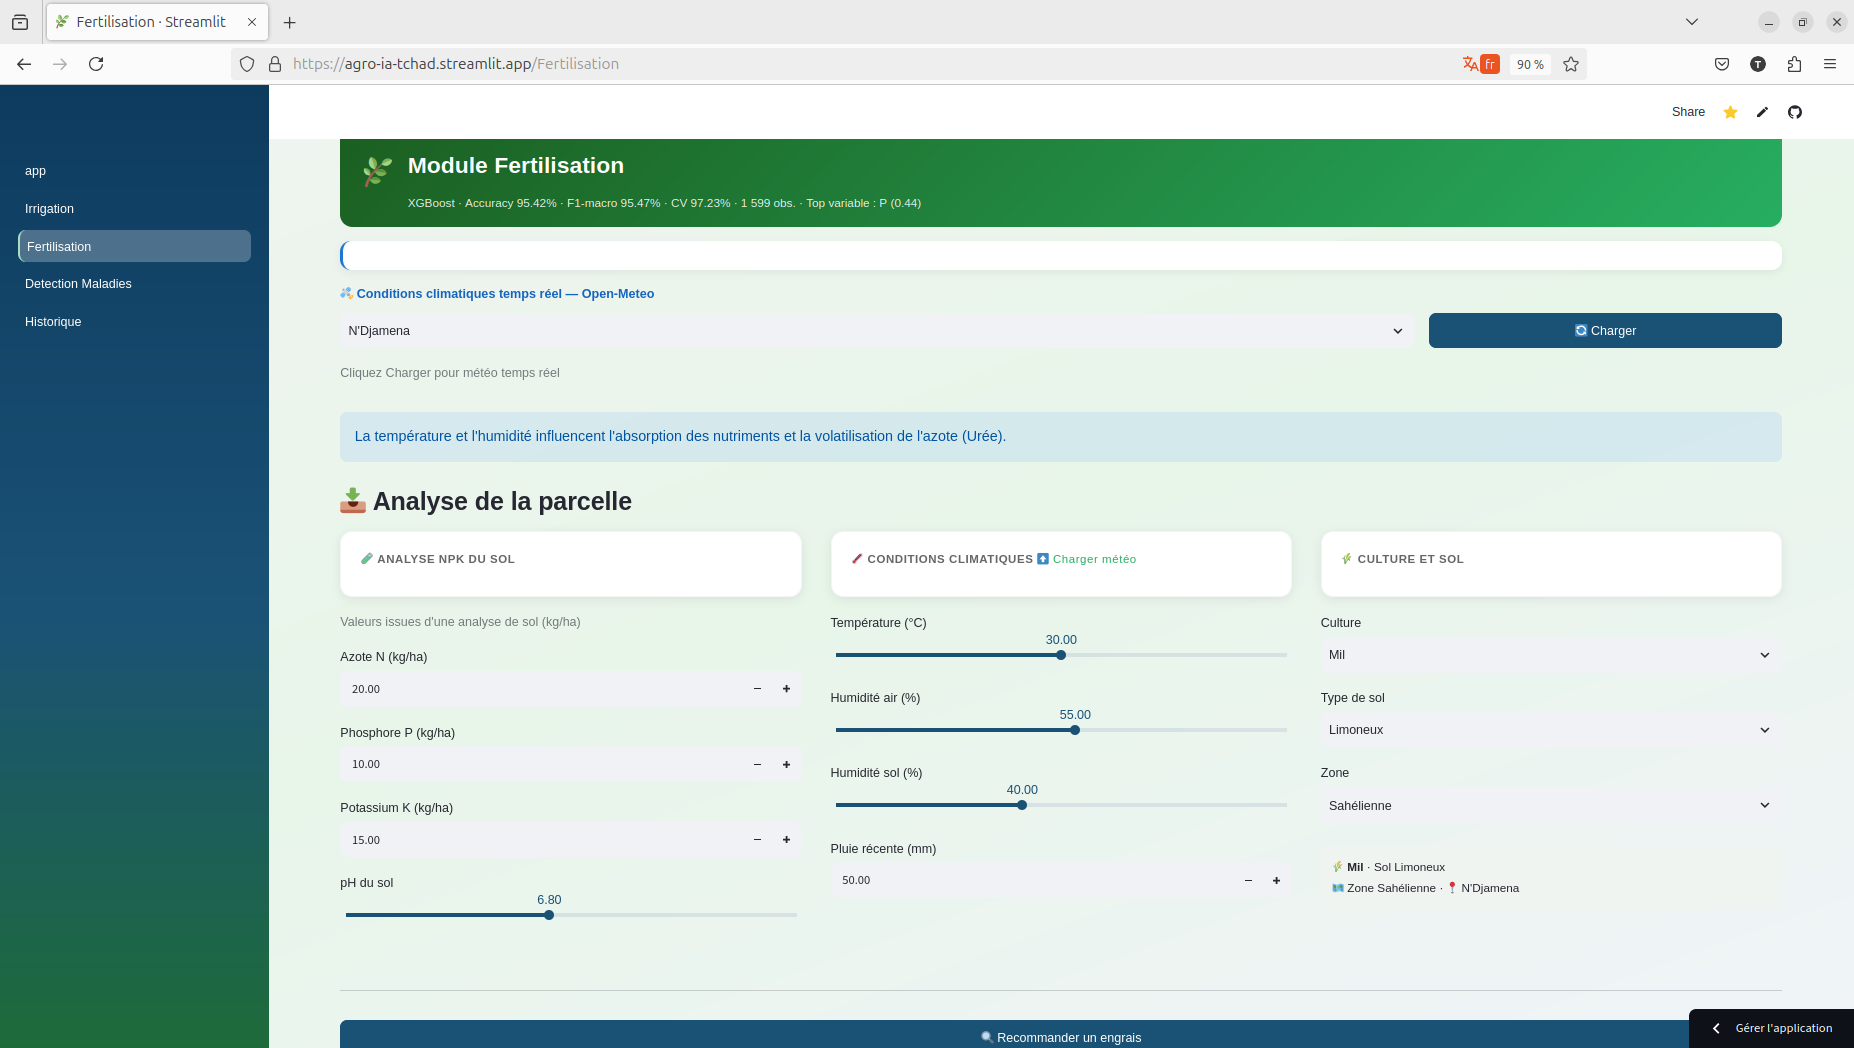
\includegraphics[width=0.9\textwidth]{images/capture_fertilisation.png}
	\fbox{\parbox{0.9\textwidth}{\centering\vspace{1.4cm}
			[Capture : module Fertilisation --- recommandation d'engrais]
			\vspace{1.4cm}}}
	\caption{Module Fertilisation --- recommandation d'engrais}
	\label{fig:cap_fert}
\end{figure}

\begin{figure}[H]
	\centering
	% 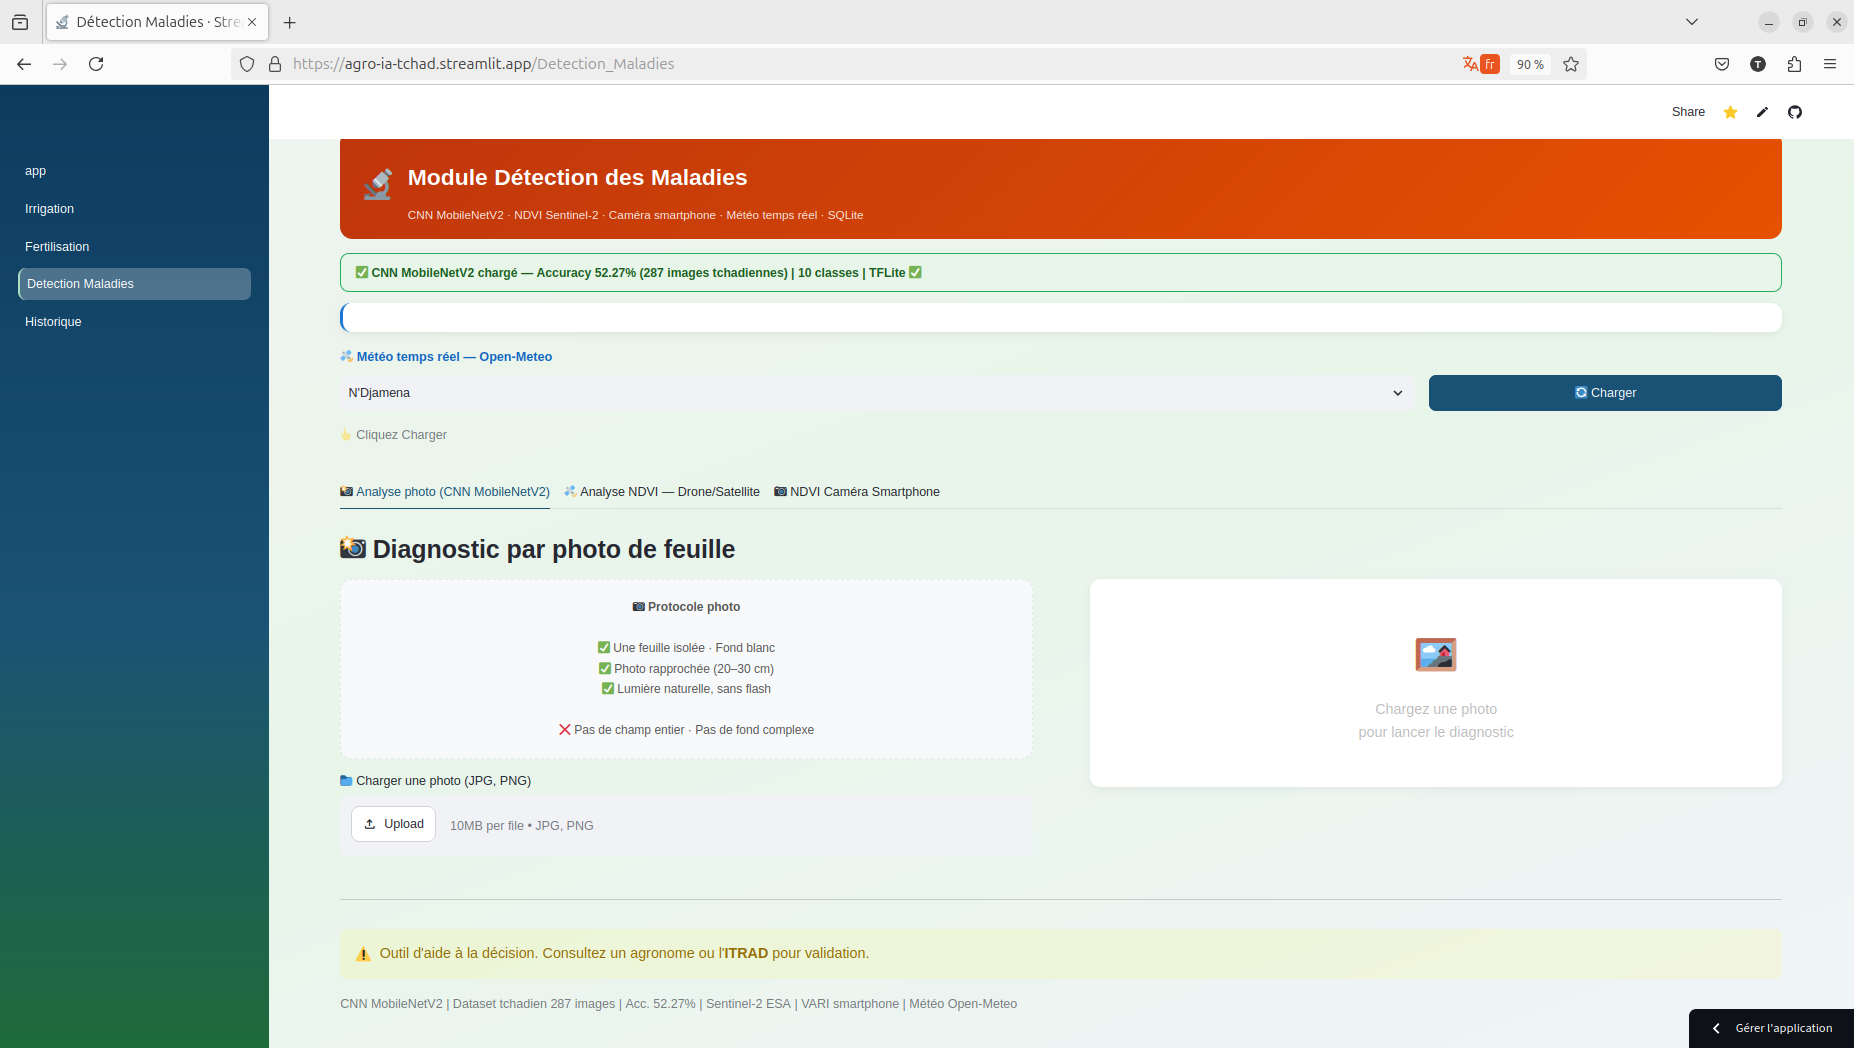
\includegraphics[width=0.9\textwidth]{images/capture_maladies.png}
	\fbox{\parbox{0.9\textwidth}{\centering\vspace{1.4cm}
			[Capture : module Maladies --- diagnostic CNN et NDVI]
			\vspace{1.4cm}}}
	\caption{Module Détection des maladies --- diagnostic par photo}
	\label{fig:cap_mal}
\end{figure}

\begin{figure}[H]
	\centering
	% 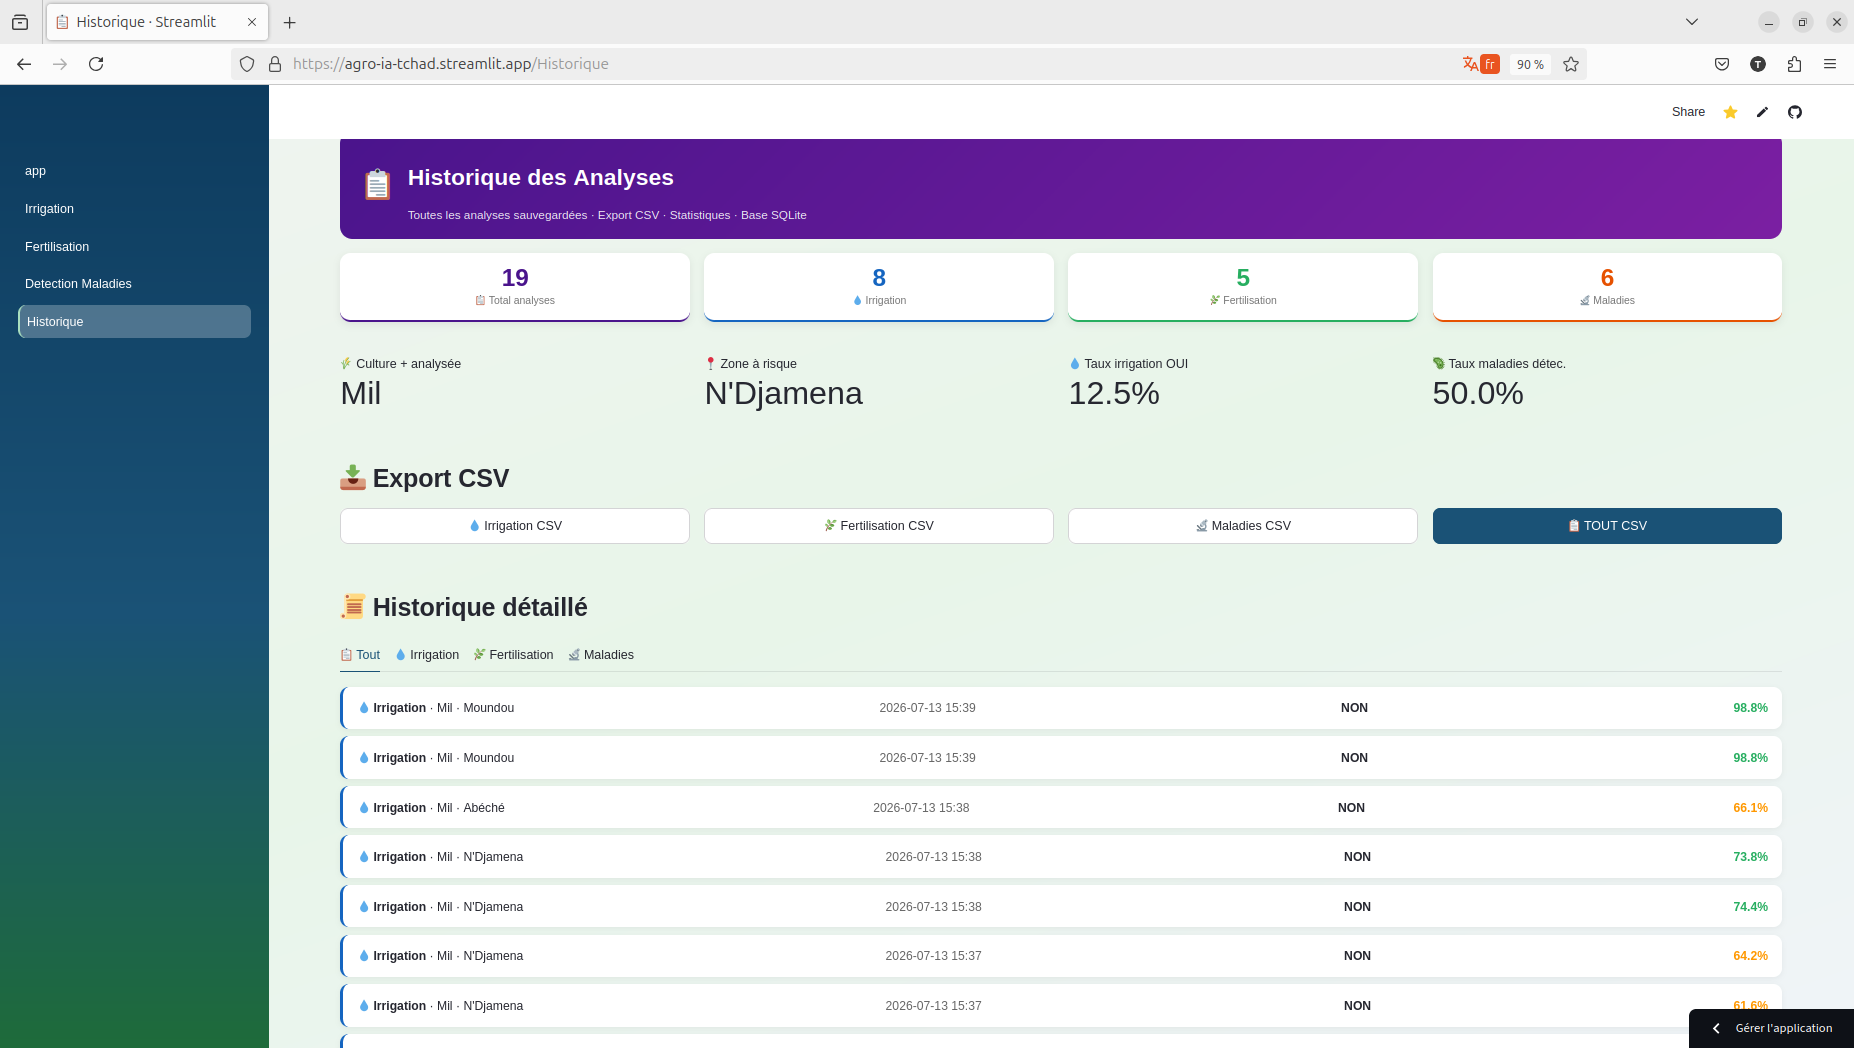
\includegraphics[width=0.9\textwidth]{images/capture_historique.png}
	\fbox{\parbox{0.9\textwidth}{\centering\vspace{1.4cm}
			[Capture : module Historique --- statistiques et export CSV]
			\vspace{1.4cm}}}
	\caption{Module Historique --- consultation et export}
	\label{fig:cap_hist}
\end{figure}